\chapter{Test Strutturale}
il test strutturale, è un tipo di test che si basa su alcuni criteri che hanno lo scopo di trovare dati di test che consentano di \textbf{percorrere tutto il programma}.

A differenza del testing funzionale, in cui la completezza del test è giudicata sui requsiti senza tener conto del programma sotto esame,
nel testing strutturale viene giudicata la completezza del test in base alla struttura del programma.

Il test strutturale è anche chiamato "white/glass box testing", mentre quello funzionale è chiamato "black box testing".

Si noti che il testing strutturale consiste ancora nel testare il prodotto (codice) rispetto alle specifiche: cambia solo la misura della completezza!

\osservazione{I test confrontano \textbf{sempre} un programma con una specifica}



\section{Adeguatezza dei test}
Quando generiamo una suite di test, come possiamo grantirne la \textbf{scrupolosità}?
Per farlo dobbiamo rispondere alle domande: 
\emph{Quali} e \emph{Quanti} test dobbiamo generare, e \emph{quando dobbiamo fermarci}.
\\In linea di principio, l'obiettivo dovrebbe essere quello di generare una suite \textbf{adeguata},
vale a dire una suite di test che, se il software sottoposto a test viene superato con successo, garantisca
una qualche proprietà del software stesso.

L'adeguatezza è quindi una sorta di "assicurazione" sull'abilità della suite di test nel trovare difetti.

\osservazione{
Non possiamo garantire in nessun modo che una suite trovi tutti o alcuni dei difetti, e non possiamo garantire neanche che li trovi con alta probabilità:
\begin{center}
    \emph{«Testing can be used to prove the presence, not the absence, of errors»}
\end{center}
}
In sostanza nessun metodo di progettazione dei test fornisce alcuna garanzia sulla capacità di scoprire difetti per le suite di test generate.

\paragraph{Cosa Facciamo?}
Quindi come costruiamo una suite di test \emph{accettabile}?
\\Generare Test randomicamente finché non finiamo tempo o budget non ci soddisfa euristicamente, utiliziamo quindi 
delle strategie basate sui \textbf{criteri di adeguatezza}.

\subsection{Criteri di Adeguatezza}
L'adeguatezza non ci da una garanzia sul potere di rilveamento dei difetti, ma é utile definire dei criteri euristici di adeguatezza simili a delle regole di progettazione.

Molte discipline progettuali utilizzano regole di progettazione per valutare \emph{non} se un progetto è adeguato, ma se \emph{esso è inadeguato}.
L'idea è che un design che segue queste rule non è necessariamente adeguato, ma uno che non segue queste regole necessariamente sarà inadeguato!

\paragraph{Criteri pratici di (in)adeguatezza per i test}
Molti criteri di (in)adeguatezza per il testing derivano da osservazioni di buon senso su ciò che ci aspetteremmo come minimo da una suite di test.

\textbf{Ricorda} che questi criteri ci aiutano a capire perchè ci piace o non piace una suite di test,
ma soddisgarli (o no) non implica niente sull'effettiva abilità della suite nel trovare difetti!

\definizione{
    Un criterio di adeguatezza è un predicato che assume valore vero o falso
    per una coppia $<P,T>$, dove $P$ è un programma e $T$ è una suite di test.
    Se il criterio è $True$, diciamo che la suite è adeguata per il programma.
}
Un criterio di adeguatezza generalmente è fatto da sottopredicati chiamati \textbf{test obligations}.

Una suite $T$ soddisfa i criteri di adeguatezza per un dato programma $P$ \emph{se e solo se}:
\begin{itemize}
    \item Tutte le esecuzioni dei casi di test in $T$ su $P$ passano.
    \item Tutte le test \textbf{obligations} sono soddisfatte da almeno un test case nella suite.
\end{itemize}

\begin{center}
    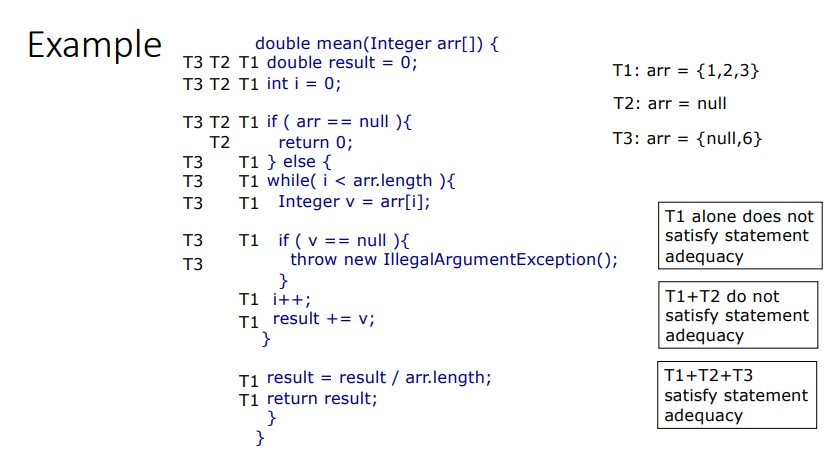
\includegraphics[width=.8\textwidth]{images/example_testing_adequacy.jpg}
\end{center}
In questo esempio abbiamo che i singoli test non riescono a soddisfare singolarmente i criteri di adeguatezza perchè non riescono a coprire l'intero codice.

%SLIDE 10


\section{Test Basato sugli Statement}
Definiamo il primo criterio di adeguatezza che guardiamo: La copertura dei Basic Block e/o degli Statement.

\subsection{Statement Coverage}

\definizione{
Per una suite di test T possiamo definire la \textbf{coverage} degli statement come la frazione di enunciati di P eseguiti da almeno un caso di test in T:
\[ C_{stmt} = \frac{\text{\# executed stmts}}{\text{\# stmts}} \]
Il test $T$ \textbf{soddisfa il criterio di adeguatezza} di statement coverage \emph{se e solo se} $C_{stmt} = 1$.
}
In sostanza, il critero di adeguatezza di statement coverage controlla quante 'righe' del codice vengono eseguite dalla suite di test, e il criterio é soddisfatto solo se tutte le righe di codice sono eseguite.

\paragraph*{Obbligazioni insoddisfacibili}
%In alcuni programmi potrebbero esistere dei criteri di adeguatezza insoddisfacibili, come ad esempio 
%alcuni statement non raggiungibili dai test.
In alcuni programmi potrebbero esistere degli statement irraggiungibili dai test, che renderebbero fisicamente insoddisfacibile il criterio di statement adequacy.
Quindi ci troveremmo delle suite che risultano inadeguate, ma soltanto perché non é fisicamente possibile renderle adeguate.
%Se non consideriamo questi elementi potremmo trovarci con delle suite che risultano inadeguate solo perché alcune obbligazioni non sono fisicamente soddisfacibili.

Bisogna quindi tenere conto di questo problema, con due approcci possibili:
\begin{itemize}
    \item Rimuovere dai criteri di adeguatezza tutte le obbligazioni di test insoddisfacibili.
    \item Usare la coverage come una misura di quanto ci siamo avvicinati all'adeguatezza.
\end{itemize}

\subsection{Basic Block Coverage}
Si puó notare che se due statements sono in sequenza, eseguirne uno automaticamente implica eseguire anche l'altro.
Quindi possiamo considerare i \textbf{basic blocks}, dove le obbligazioni sono i blocchi del CFG\footnote{Control Flow Graph} del programma.

\definizione{Un Basic Block è una sequenza massima di istruzioni di programma contigue con un punto di ingresso e un punto di uscita.}

\subsubsection{Control Flow Graph}
Come si costruisce un CFG?
Un Control Flow Graph per un programma $P$ é un grafo con:
\begin{itemize}
    \item \textbf{Nodi} che rappresentano i Basic Blocks di $P$
    \item \textbf{Edges} che connettono i BB in una relazione sequenziale, possono essere etichettati con T o F se il BB finisce con un controllo condizionale
\end{itemize}

\subsection{BB/Stmt Adeuqacy Rationale}

\subsection{Test suit Size VS Coverage}

\section{Test basato sui Branch}

\section{Test basato sulle Condizioni}